\documentclass[12pt]{exam}
\usepackage[portuguese]{babel}
\usepackage[utf8]{inputenc}
\usepackage{graphicx}
\graphicspath{{figuras/}}

\usepackage[margin=1in]{geometry}
\usepackage{amsmath,amssymb}
\usepackage{multicol}

\newcommand{\disciplina}{Banco de Dados}
\newcommand{\class}{\disciplina}
\newcommand{\term}{Professor: Igor Avila Pereira}
\newcommand{\bimestre}{1}
\newcommand{\valor}{4}
\newcommand{\examnum}{Prova \bimestreº Bim. - Valor: \valor}
%\newcommand{\examdate}{xx}
%\newcommand{\timelimit}{4 horas}

\pagestyle{head}
\firstpageheader{}{}{}
\runningheader{\class} - {Página \thepage\ de \numpages}
\runningheadrule

\begin{document}

\noindent
\begin{tabular*}{\textwidth}{l @{\extracolsep{\fill}} r @{\extracolsep{6pt}} l}
\textbf{\class} & \textbf{Nome:} & \makebox[2in]{\hrulefill}   \\
\textbf{\examnum} & \textbf{Matrícula:} & \makebox[2in]{\hrulefill}   \\
%\textbf{\examnum} &&\\
%\textbf{\examdate} &&\\
\textbf{\term} &&\\
%\textbf{Duração: \timelimit}
\end{tabular*}\\
\rule[2ex]{\textwidth}{2pt}
\noindent
%rule[2ex]{\textwidth}{2pt}

\begin{questions}

\question Um escritório de advocacia deseja construir um banco de dados para armazenar dados de clientes, processos e advogados. Para cada cliente deseja-se registrar um código, nome, CPF, telefone para contato e endereço. Para cada processo, deseja-se guardar um código, data de abertura e descrição. Cada processo será aberto por um cliente e pode ser atendido por um ou mais advogados. Para cada advogado deseja-se registrar um código, nome, telefone, data de entrada na empresa e número de registro na OAB. Para cada processo devem ser armazenados também os dados de cada audiência relacionada a ele (um código, data, hora e local). 
\textbf{Faça um modelo ER para este banco de dados.}
\label{ER-Exercicio-direito}


\begin{figure}[!ht]
	\centering
	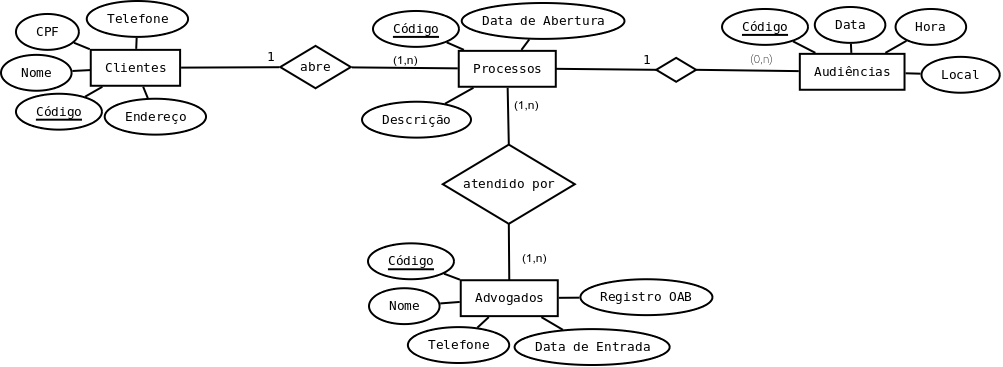
\includegraphics[width=1\linewidth]{figuras/ER-Exercicio-direito.png}
	\caption{Gabarito - Exercício \ref{ER-Exercicio-direito}.}
\end{figure}


\newpage

\question\textbf{ Construa um diagrama ER} para uma seguradora de automóveis em que cada cliente possui um ou mais carros. Cada carro tem associado a ele zero a qualquer número de acidentes registrados. Para cada cliente é necessário registrar seu nome, CPF, número da CNH, endereço e telefone. Para cada carro, é necessário registrar uma descrição, número da placa, número do chassi e quantidade de quilômetros rodados. Para cada acidente registrar uma descrição, data, hora, local, e valor total dos danos. 
\label{ER-Exercicio-seguradora-automoveis}

\begin{figure}[!ht]
\centering
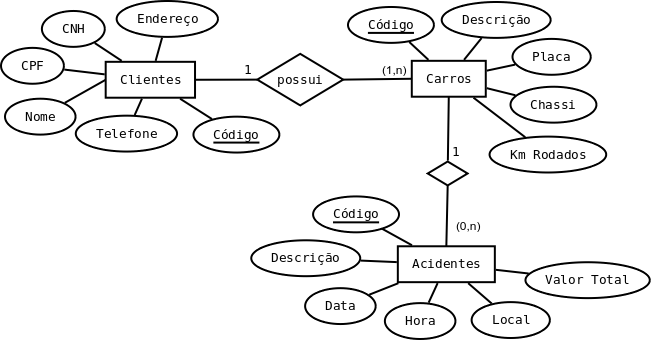
\includegraphics[width=0.9\linewidth]{figuras/ER-Exercicio-seguradora-automoveis.png}
\caption{Gabarito - Exercício \ref{ER-Exercicio-seguradora-automoveis}.}
\end{figure}

\newpage

\question Uma universidade deseja construir um banco de dados para armazenar o QSL (Quadro de Sequência Lógica) de cada curso ofertado por ela. Todos os cursos nessa universidade são semestrais. Para cada curso, deseja-se armazenar as seguintes informações: código do curso, nome, turno (diurno ou noturno) e nível (graduação, especialização, mestrado ou doutorado). Cada curso é mantido por um departamento. Para cada departamento deve ser registrados seu código e nome. Para cada curso existe um conjunto de uma ou mais disciplinas. Para cada disciplina devem ser armazenados: um código, nome, créditos, carga horária total, ementa e o número do semestre de oferecimento. Cada disciplina também possui zero ou mais pré-requisitos, que são disciplinas que um determinado aluno deve ter concluído para poder se matricular na disciplina em questão. 
\textbf{Faça um modelo ER para este banco de dados.}
\label{ER-Exercicio-universidade}

\begin{figure}[!htp]
\centering
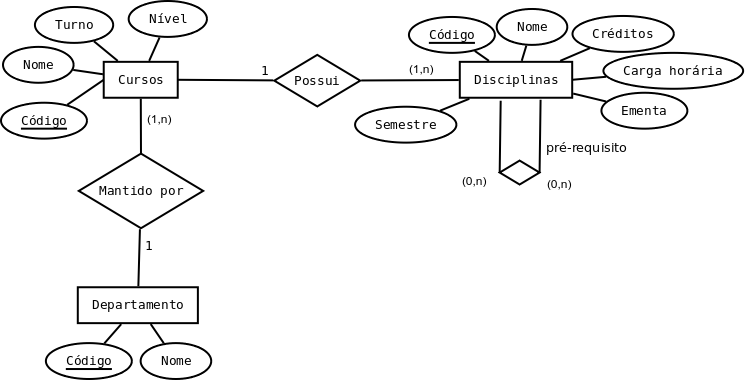
\includegraphics[width=1\linewidth]{figuras/ER-Exercicio-universidade.png}
\caption{Gabarito - Exercício \ref{ER-Exercicio-universidade}.}
\end{figure}

\newpage

\question \textbf{Construa um diagrama ER} para um hospital, onde se deseja armazenar dados sobre pacientes, exames e médicos. Para cada paciente, devem ser guardados seu nome, CPF, RG, data de nascimento, endereço e telefone. Para cada médico deseja-se guardar seu nome, telefone e número de registro no CRM (Conselho Regional de Medicina). Cada médico pode possuir uma ou mais especialidades. Para cada especialidade deve-se armazenar um código e um nome. Também deseja-se manter um registro de exames feitos por cada paciente. O exame deverá ser requisitado por um médico. Para cada exame deve-se registrar data e hora de realização, valor e uma descrição do mesmo.  \label{ER-Exercicio-hospital}

\begin{figure}[!htp]
\centering
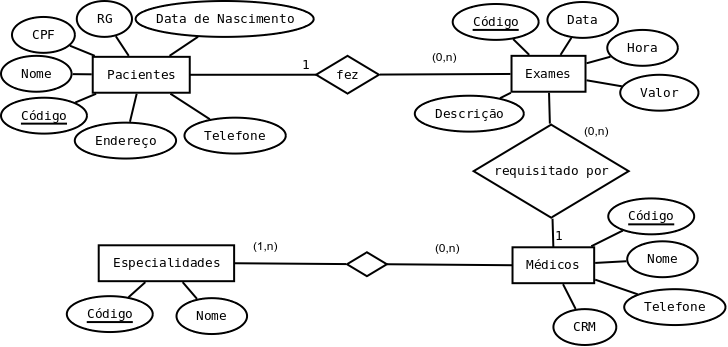
\includegraphics[width=1\linewidth]{figuras/ER-Exercicio-hospital.png}
\caption{Gabarito - Exercício \ref{ER-Exercicio-hospital}.}
\end{figure}

\end{questions}
\end{document}